% 赵爽弦图：四个直角三角形拼大正方形, 中间小正方形
\documentclass[tikz,border=4pt]{standalone}
\usepackage{ctex}
\usepackage{amsmath}
\begin{document}
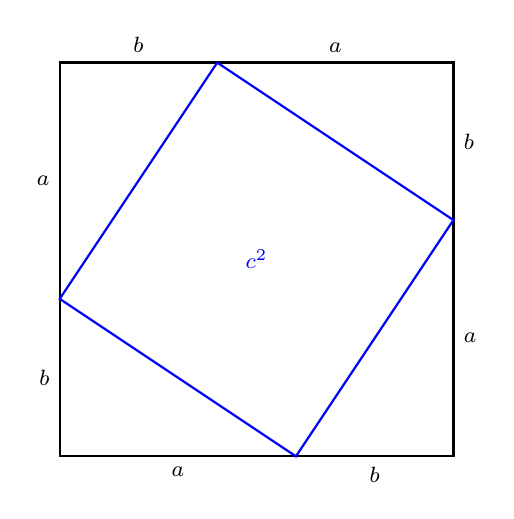
\begin{tikzpicture}[scale=1.0, thick]
  % 大正方形边长 5（a=3, b=4, c=5）
  \draw (0,0) -- (5,0) -- (5,5) -- (0,5) -- cycle;
  % 内部小正方形（旋转）由四个三角形围成
  % 4 个直角顶点：把每边按 3:2 分（不对，按 a:b 分使内部正方形边 = c-... 这里用 a=3, b=4, c=5 简化为视觉示意）
  % 关键：从每个边出发，沿边 a=3 的点
  \coordinate (P1) at (3, 0);
  \coordinate (P2) at (5, 3);
  \coordinate (P3) at (2, 5);
  \coordinate (P4) at (0, 2);
  \draw[blue] (P1) -- (P2) -- (P3) -- (P4) -- cycle;
  % 4 个直角三角形对角线（已经画了边）
  % 标记
  \node[below] at (1.5, 0) {\footnotesize $a$};
  \node[below] at (4, 0)   {\footnotesize $b$};
  \node[right] at (5, 1.5) {\footnotesize $a$};
  \node[right] at (5, 4)   {\footnotesize $b$};
  \node[above] at (3.5, 5) {\footnotesize $a$};
  \node[above] at (1, 5)   {\footnotesize $b$};
  \node[left]  at (0, 3.5) {\footnotesize $a$};
  \node[left]  at (0, 1)   {\footnotesize $b$};
  \node[blue]  at (2.5, 2.5) {\footnotesize $c^2$};
\end{tikzpicture}
\end{document}
